\documentclass[twoside]{book}

% Packages required by doxygen
\usepackage{fixltx2e}
\usepackage{calc}
\usepackage{doxygen}
\usepackage[export]{adjustbox} % also loads graphicx
\usepackage{graphicx}
\usepackage[utf8]{inputenc}
\usepackage{makeidx}
\usepackage{multicol}
\usepackage{multirow}
\PassOptionsToPackage{warn}{textcomp}
\usepackage{textcomp}
\usepackage[nointegrals]{wasysym}
\usepackage[table]{xcolor}

% Font selection
\usepackage[T1]{fontenc}
\usepackage[scaled=.90]{helvet}
\usepackage{courier}
\usepackage{amssymb}
\usepackage{sectsty}
\renewcommand{\familydefault}{\sfdefault}
\allsectionsfont{%
  \fontseries{bc}\selectfont%
  \color{darkgray}%
}
\renewcommand{\DoxyLabelFont}{%
  \fontseries{bc}\selectfont%
  \color{darkgray}%
}
\newcommand{\+}{\discretionary{\mbox{\scriptsize$\hookleftarrow$}}{}{}}

% Page & text layout
\usepackage{geometry}
\geometry{%
  a4paper,%
  top=2.5cm,%
  bottom=2.5cm,%
  left=2.5cm,%
  right=2.5cm%
}
\tolerance=750
\hfuzz=15pt
\hbadness=750
\setlength{\emergencystretch}{15pt}
\setlength{\parindent}{0cm}
\setlength{\parskip}{3ex plus 2ex minus 2ex}
\makeatletter
\renewcommand{\paragraph}{%
  \@startsection{paragraph}{4}{0ex}{-1.0ex}{1.0ex}{%
    \normalfont\normalsize\bfseries\SS@parafont%
  }%
}
\renewcommand{\subparagraph}{%
  \@startsection{subparagraph}{5}{0ex}{-1.0ex}{1.0ex}{%
    \normalfont\normalsize\bfseries\SS@subparafont%
  }%
}
\makeatother

% Headers & footers
\usepackage{fancyhdr}
\pagestyle{fancyplain}
\fancyhead[LE]{\fancyplain{}{\bfseries\thepage}}
\fancyhead[CE]{\fancyplain{}{}}
\fancyhead[RE]{\fancyplain{}{\bfseries\leftmark}}
\fancyhead[LO]{\fancyplain{}{\bfseries\rightmark}}
\fancyhead[CO]{\fancyplain{}{}}
\fancyhead[RO]{\fancyplain{}{\bfseries\thepage}}
\fancyfoot[LE]{\fancyplain{}{}}
\fancyfoot[CE]{\fancyplain{}{}}
\fancyfoot[RE]{\fancyplain{}{\bfseries\scriptsize Generated by Doxygen }}
\fancyfoot[LO]{\fancyplain{}{\bfseries\scriptsize Generated by Doxygen }}
\fancyfoot[CO]{\fancyplain{}{}}
\fancyfoot[RO]{\fancyplain{}{}}
\renewcommand{\footrulewidth}{0.4pt}
\renewcommand{\chaptermark}[1]{%
  \markboth{#1}{}%
}
\renewcommand{\sectionmark}[1]{%
  \markright{\thesection\ #1}%
}

% Indices & bibliography
\usepackage{natbib}
\usepackage[titles]{tocloft}
\setcounter{tocdepth}{3}
\setcounter{secnumdepth}{5}
\makeindex

% Hyperlinks (required, but should be loaded last)
\usepackage{ifpdf}
\ifpdf
  \usepackage[pdftex,pagebackref=true]{hyperref}
\else
  \usepackage[ps2pdf,pagebackref=true]{hyperref}
\fi
\hypersetup{%
  colorlinks=true,%
  linkcolor=blue,%
  citecolor=blue,%
  unicode%
}

% Custom commands
\newcommand{\clearemptydoublepage}{%
  \newpage{\pagestyle{empty}\cleardoublepage}%
}

\usepackage{caption}
\captionsetup{labelsep=space,justification=centering,font={bf},singlelinecheck=off,skip=4pt,position=top}

%===== C O N T E N T S =====

\begin{document}

% Titlepage & ToC
\hypersetup{pageanchor=false,
             bookmarksnumbered=true,
             pdfencoding=unicode
            }
\pagenumbering{alph}
\begin{titlepage}
\vspace*{7cm}
\begin{center}%
{\Large Stack\+\_\+int \\[1ex]\large 1.\+0 }\\
\vspace*{1cm}
{\large Generated by Doxygen 1.8.13}\\
\end{center}
\end{titlepage}
\clearemptydoublepage
\pagenumbering{roman}
\tableofcontents
\clearemptydoublepage
\pagenumbering{arabic}
\hypersetup{pageanchor=true}

%--- Begin generated contents ---
\chapter{Todo List}
\label{todo}
\Hypertarget{todo}

\begin{DoxyRefList}
\item[\label{todo__todo000001}%
\Hypertarget{todo__todo000001}%
File \hyperlink{main_8cpp}{main.cpp} ]
\end{DoxyRefList}
\chapter{Class Index}
\section{Class List}
Here are the classes, structs, unions and interfaces with brief descriptions\+:\begin{DoxyCompactList}
\item\contentsline{section}{\hyperlink{struct_stack}{Stack} \\*\hyperlink{struct_stack}{Stack} structure }{\pageref{struct_stack}}{}
\end{DoxyCompactList}

\chapter{File Index}
\section{File List}
Here is a list of all documented files with brief descriptions\+:\begin{DoxyCompactList}
\item\contentsline{section}{\hyperlink{main_8cpp}{main.\+cpp} \\*Третье домашнее задание по курсу \char`\"{}Введение в промышленное программирование и структуры данных\char`\"{} }{\pageref{main_8cpp}}{}
\end{DoxyCompactList}

\chapter{Class Documentation}
\hypertarget{struct_stack}{}\section{Stack Struct Reference}
\label{struct_stack}\index{Stack@{Stack}}


\hyperlink{struct_stack}{Stack} structure.  


\subsection*{Public Attributes}
\begin{DoxyCompactItemize}
\item 
\mbox{\Hypertarget{struct_stack_a7361bb8e21c53fc8660de4b91a382a99}\label{struct_stack_a7361bb8e21c53fc8660de4b91a382a99}} 
uint16\+\_\+t {\bfseries canary1} = 0x\+B\+E\+DA
\item 
\mbox{\Hypertarget{struct_stack_ae3c965578ef7a6d060e8178346d519d4}\label{struct_stack_ae3c965578ef7a6d060e8178346d519d4}} 
unsigned \hyperlink{struct_stack_ae3c965578ef7a6d060e8178346d519d4}{count} = 0
\begin{DoxyCompactList}\small\item\em control element for penetration protection \end{DoxyCompactList}\item 
\mbox{\Hypertarget{struct_stack_a0c2c0c7f1d93b40c1dca5e6c104a029e}\label{struct_stack_a0c2c0c7f1d93b40c1dca5e6c104a029e}} 
unsigned \hyperlink{struct_stack_a0c2c0c7f1d93b40c1dca5e6c104a029e}{capacity} = 0
\begin{DoxyCompactList}\small\item\em stack count \end{DoxyCompactList}\item 
\mbox{\Hypertarget{struct_stack_ae78a95cf617c377a5f12d556d2b620e3}\label{struct_stack_ae78a95cf617c377a5f12d556d2b620e3}} 
long unsigned \hyperlink{struct_stack_ae78a95cf617c377a5f12d556d2b620e3}{stk\+\_\+sum} = 0
\begin{DoxyCompactList}\small\item\em stack volume \end{DoxyCompactList}\item 
\mbox{\Hypertarget{struct_stack_a0c78ec8c4ec1de7a2a49f210a05031e4}\label{struct_stack_a0c78ec8c4ec1de7a2a49f210a05031e4}} 
long unsigned \hyperlink{struct_stack_a0c78ec8c4ec1de7a2a49f210a05031e4}{dat\+\_\+sum} = 0
\begin{DoxyCompactList}\small\item\em stack structure checksum \end{DoxyCompactList}\item 
\mbox{\Hypertarget{struct_stack_a67fb5cb41d557b98e5a8cd5699e1ba8f}\label{struct_stack_a67fb5cb41d557b98e5a8cd5699e1ba8f}} 
unsigned $\ast$ \hyperlink{struct_stack_a67fb5cb41d557b98e5a8cd5699e1ba8f}{data} = static\+\_\+cast$<$unsigned$\ast$$>$(nullptr)
\begin{DoxyCompactList}\small\item\em data array ckecksum \end{DoxyCompactList}\item 
\mbox{\Hypertarget{struct_stack_ae3b5cfcce1d3f0c6e281600a5a4ce0ea}\label{struct_stack_ae3b5cfcce1d3f0c6e281600a5a4ce0ea}} 
unsigned $\ast$ \hyperlink{struct_stack_ae3b5cfcce1d3f0c6e281600a5a4ce0ea}{dat\+\_\+can1} = static\+\_\+cast$<$unsigned$\ast$$>$(nullptr)
\begin{DoxyCompactList}\small\item\em data aray pointer \end{DoxyCompactList}\item 
\mbox{\Hypertarget{struct_stack_acde7d81e3217c8585cfc5dfc89bf8365}\label{struct_stack_acde7d81e3217c8585cfc5dfc89bf8365}} 
unsigned $\ast$ \hyperlink{struct_stack_acde7d81e3217c8585cfc5dfc89bf8365}{dat\+\_\+can2} = static\+\_\+cast$<$unsigned$\ast$$>$(nullptr)
\begin{DoxyCompactList}\small\item\em control element pointer \end{DoxyCompactList}\item 
\mbox{\Hypertarget{struct_stack_a4b90f612738df33e56b75796d0525912}\label{struct_stack_a4b90f612738df33e56b75796d0525912}} 
uint16\+\_\+t \hyperlink{struct_stack_a4b90f612738df33e56b75796d0525912}{canary2} = 0x\+B\+E\+DA
\begin{DoxyCompactList}\small\item\em control element pointer \end{DoxyCompactList}\end{DoxyCompactItemize}


\subsection{Detailed Description}
\hyperlink{struct_stack}{Stack} structure. 

The documentation for this struct was generated from the following file\+:\begin{DoxyCompactItemize}
\item 
\hyperlink{main_8cpp}{main.\+cpp}\end{DoxyCompactItemize}

\chapter{File Documentation}
\hypertarget{main_8cpp}{}\section{main.\+cpp File Reference}
\label{main_8cpp}\index{main.\+cpp@{main.\+cpp}}


Третье домашнее задание по курсу \char`\"{}Введение в промышленное программирование и структуры данных\char`\"{}.  


{\ttfamily \#include $<$iostream$>$}\newline
{\ttfamily \#include $<$cassert$>$}\newline
{\ttfamily \#include $<$cstring$>$}\newline
{\ttfamily \#include $<$cstdlib$>$}\newline
Include dependency graph for main.\+cpp\+:\nopagebreak
\begin{figure}[H]
\begin{center}
\leavevmode
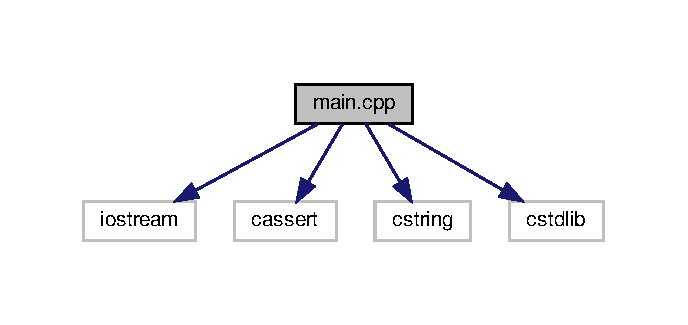
\includegraphics[width=330pt]{main_8cpp__incl}
\end{center}
\end{figure}
\subsection*{Classes}
\begin{DoxyCompactItemize}
\item 
struct \hyperlink{struct_stack}{Stack}
\begin{DoxyCompactList}\small\item\em \hyperlink{struct_stack}{Stack} structure. \end{DoxyCompactList}\end{DoxyCompactItemize}
\subsection*{Macros}
\begin{DoxyCompactItemize}
\item 
\#define \hyperlink{main_8cpp_af78f5d96888ec5049f9fefde0706fec9}{U\+N\+I\+T\+T\+E\+ST}(what,  op,  ref)
\begin{DoxyCompactList}\small\item\em Unit test define. \end{DoxyCompactList}\item 
\#define \hyperlink{main_8cpp_a92393412e72b674676ff5cd2cd9cefdf}{Stack\+\_\+dump}(inp\+St,  reason)
\begin{DoxyCompactList}\small\item\em Prints full stack dump. \end{DoxyCompactList}\item 
\#define \hyperlink{main_8cpp_a9962d82f01e3d36f8f7969c50f9e46b8}{A\+S\+S\+E\+R\+T\+\_\+\+OK}(inp\+St,  reason)~if(\hyperlink{main_8cpp_a4d7881c343dba87c78ae6bd2a303ee15}{Stack\+\_\+\+OK}(inp\+St) != 0) \{\hyperlink{main_8cpp_a92393412e72b674676ff5cd2cd9cefdf}{Stack\+\_\+dump}(inp\+St, reason); assert(!reason);\}
\begin{DoxyCompactList}\small\item\em Checks if stack is damaged. \end{DoxyCompactList}\end{DoxyCompactItemize}
\subsection*{Functions}
\begin{DoxyCompactItemize}
\item 
long unsigned \hyperlink{main_8cpp_a1322b76738bcc52bee44ba55829006ef}{calc\+\_\+stk\+\_\+sum} (\hyperlink{struct_stack}{Stack} $\ast$inp\+St)
\begin{DoxyCompactList}\small\item\em Calculates control sum of the stack. \end{DoxyCompactList}\item 
long unsigned \hyperlink{main_8cpp_a7af33ef8ba5d5eff8b77286245ceaf6e}{calc\+\_\+dat\+\_\+sum} (\hyperlink{struct_stack}{Stack} $\ast$inp\+St)
\begin{DoxyCompactList}\small\item\em Calculates control sum of the data aray. \end{DoxyCompactList}\item 
void \hyperlink{main_8cpp_aa48f8c7b961d5a02093e377f661c7b7f}{write\+\_\+stk\+\_\+sum} (\hyperlink{struct_stack}{Stack} $\ast$inp\+St)
\begin{DoxyCompactList}\small\item\em Writes checksum of the stack. \end{DoxyCompactList}\item 
void \hyperlink{main_8cpp_a73b897a8ca5ac21acff9cc206b95b631}{write\+\_\+dat\+\_\+sum} (\hyperlink{struct_stack}{Stack} $\ast$inp\+St)
\begin{DoxyCompactList}\small\item\em Writes checksum of the data aray. \end{DoxyCompactList}\item 
void \hyperlink{main_8cpp_a2ecb86ff492da6c341c3a4dde7061bc4}{write\+\_\+control\+\_\+sums} (\hyperlink{struct_stack}{Stack} $\ast$inp\+St)
\begin{DoxyCompactList}\small\item\em Writes checksums of the stack and data aray. \end{DoxyCompactList}\item 
int \hyperlink{main_8cpp_a4d7881c343dba87c78ae6bd2a303ee15}{Stack\+\_\+\+OK} (\hyperlink{struct_stack}{Stack} $\ast$inp\+St)
\begin{DoxyCompactList}\small\item\em Quiet verification of the stack. \end{DoxyCompactList}\item 
void \hyperlink{main_8cpp_a67d8f7547eee1472c01d20971401654a}{create\+\_\+new\+\_\+data} (\hyperlink{struct_stack}{Stack} $\ast$inp\+St)
\begin{DoxyCompactList}\small\item\em Creates new data aray. \end{DoxyCompactList}\item 
void \hyperlink{main_8cpp_aa40da29b3a5ffeccd6999affe725e450}{Stack\+Ctor} (\hyperlink{struct_stack}{Stack} $\ast$inp\+St)
\begin{DoxyCompactList}\small\item\em Creates new stack from inp\+St. \end{DoxyCompactList}\item 
\hyperlink{struct_stack}{Stack} \hyperlink{main_8cpp_adce6355a7341f2c2802290c7cb5936d2}{Stack\+New} ()
\begin{DoxyCompactList}\small\item\em Creates new stack from nothing. \end{DoxyCompactList}\item 
void \hyperlink{main_8cpp_a78f4cf4dab35251303dad715b0ce935a}{poison\+\_\+dat} (\hyperlink{struct_stack}{Stack} $\ast$inp\+St)
\begin{DoxyCompactList}\small\item\em Poisons all data aray elements (assigns with 666) \end{DoxyCompactList}\item 
void \hyperlink{main_8cpp_abe4787c06681c2320e30629a1089719b}{poison\+\_\+stk} (\hyperlink{struct_stack}{Stack} $\ast$inp\+St)
\begin{DoxyCompactList}\small\item\em Poisons all stack structure members (assigns with 666) \end{DoxyCompactList}\item 
void \hyperlink{main_8cpp_a77f28da6fc285875bf4281869c320720}{Stack\+Dtor} (\hyperlink{struct_stack}{Stack} $\ast$inp\+St)
\begin{DoxyCompactList}\small\item\em Destructes the stack. \end{DoxyCompactList}\item 
void \hyperlink{main_8cpp_a312803b8f2fd6047156a464c05943f3c}{expand\+\_\+stk} (\hyperlink{struct_stack}{Stack} $\ast$inp\+St, uint8\+\_\+t is\+Exp)
\begin{DoxyCompactList}\small\item\em Expands stack (makes twice larger or twice smaller) \end{DoxyCompactList}\item 
void \hyperlink{main_8cpp_a9441c68501c4b28326feb25b3dfbd2c4}{Push\+\_\+back} (\hyperlink{struct_stack}{Stack} $\ast$inp\+St, unsigned val)
\begin{DoxyCompactList}\small\item\em Pushes val to the top of the stack. \end{DoxyCompactList}\item 
unsigned \hyperlink{main_8cpp_a17cb699dcfc7c06b3d2d9ebbe756bb8b}{Pop\+\_\+back} (\hyperlink{struct_stack}{Stack} $\ast$inp\+St)
\begin{DoxyCompactList}\small\item\em Pops element from the top of the stack. \end{DoxyCompactList}\item 
void \hyperlink{main_8cpp_a10c018abd2bff2ae8f7ea819c5cd3581}{My\+\_\+dump} (\hyperlink{struct_stack}{Stack} $\ast$inp\+St)
\begin{DoxyCompactList}\small\item\em My version of stack dump. \end{DoxyCompactList}\item 
unsigned \hyperlink{main_8cpp_a844584f19d99f328035955f8e215a0f3}{Stack\+Size} (\hyperlink{struct_stack}{Stack} $\ast$inp\+St)
\begin{DoxyCompactList}\small\item\em Returns size of the stack. \end{DoxyCompactList}\item 
unsigned \hyperlink{main_8cpp_a68b4940ac8f933d0f2412c9e3a253547}{Stack\+Capacity} (\hyperlink{struct_stack}{Stack} $\ast$inp\+St)
\begin{DoxyCompactList}\small\item\em Returns volume of the stack. \end{DoxyCompactList}\item 
double \hyperlink{main_8cpp_a9a6bcc2b1abd29f189a03ee990a36177}{Stack\+Top} (\hyperlink{struct_stack}{Stack} $\ast$inp\+St)
\begin{DoxyCompactList}\small\item\em Returns top element of the stack without removing it. \end{DoxyCompactList}\item 
\mbox{\Hypertarget{main_8cpp_ae66f6b31b5ad750f1fe042a706a4e3d4}\label{main_8cpp_ae66f6b31b5ad750f1fe042a706a4e3d4}} 
int {\bfseries main} ()
\end{DoxyCompactItemize}


\subsection{Detailed Description}
Третье домашнее задание по курсу \char`\"{}Введение в промышленное программирование и структуры данных\char`\"{}. 

\begin{DoxyAuthor}{Author}
Philip Khristolyubov 
\end{DoxyAuthor}
\begin{DoxyVersion}{Version}
1.\+0 
\end{DoxyVersion}
\begin{DoxyDate}{Date}
01.\+11.\+2018 
\end{DoxyDate}
\begin{DoxyRefDesc}{Todo}
\item[\hyperlink{todo__todo000001}{Todo}]\end{DoxyRefDesc}


\subsection{Macro Definition Documentation}
\mbox{\Hypertarget{main_8cpp_a9962d82f01e3d36f8f7969c50f9e46b8}\label{main_8cpp_a9962d82f01e3d36f8f7969c50f9e46b8}} 
\index{main.\+cpp@{main.\+cpp}!A\+S\+S\+E\+R\+T\+\_\+\+OK@{A\+S\+S\+E\+R\+T\+\_\+\+OK}}
\index{A\+S\+S\+E\+R\+T\+\_\+\+OK@{A\+S\+S\+E\+R\+T\+\_\+\+OK}!main.\+cpp@{main.\+cpp}}
\subsubsection{\texorpdfstring{A\+S\+S\+E\+R\+T\+\_\+\+OK}{ASSERT\_OK}}
{\footnotesize\ttfamily \#define A\+S\+S\+E\+R\+T\+\_\+\+OK(\begin{DoxyParamCaption}\item[{}]{inp\+St,  }\item[{}]{reason }\end{DoxyParamCaption})~if(\hyperlink{main_8cpp_a4d7881c343dba87c78ae6bd2a303ee15}{Stack\+\_\+\+OK}(inp\+St) != 0) \{\hyperlink{main_8cpp_a92393412e72b674676ff5cd2cd9cefdf}{Stack\+\_\+dump}(inp\+St, reason); assert(!reason);\}}



Checks if stack is damaged. 


\begin{DoxyParams}{Parameters}
{\em inp\+St} & poiner to stack for dump \\
\hline
{\em reason} & reason why do you use dump (reason will be printed before dump) \\
\hline
\end{DoxyParams}
\mbox{\Hypertarget{main_8cpp_a92393412e72b674676ff5cd2cd9cefdf}\label{main_8cpp_a92393412e72b674676ff5cd2cd9cefdf}} 
\index{main.\+cpp@{main.\+cpp}!Stack\+\_\+dump@{Stack\+\_\+dump}}
\index{Stack\+\_\+dump@{Stack\+\_\+dump}!main.\+cpp@{main.\+cpp}}
\subsubsection{\texorpdfstring{Stack\+\_\+dump}{Stack\_dump}}
{\footnotesize\ttfamily \#define Stack\+\_\+dump(\begin{DoxyParamCaption}\item[{}]{inp\+St,  }\item[{}]{reason }\end{DoxyParamCaption})}

{\bfseries Value\+:}
\begin{DoxyCode}
\{\(\backslash\)
    auto addr = (inpSt);\(\backslash\)
    auto res = \hyperlink{main_8cpp_a4d7881c343dba87c78ae6bd2a303ee15}{Stack\_OK}(inpSt);\(\backslash\)
    cout << \textcolor{stringliteral}{"-------------------------------------------------------"} << endl;\(\backslash\)
    cout << (reason) << endl;\(\backslash\)
    cout << \textcolor{stringliteral}{"Stack "} << #inpSt << \textcolor{stringliteral}{" "} << addr << \textcolor{stringliteral}{" Stack\_OK:"} << res << endl;\(\backslash\)
    cout << \textcolor{stringliteral}{"Capacity: "} << inpSt->capacity << endl;\(\backslash\)
    cout << \textcolor{stringliteral}{"Count: "} << inpSt->count << endl;\(\backslash\)
    cout << \textcolor{stringliteral}{"Data: "} << inpSt->data << endl;\(\backslash\)
    cout << \textcolor{stringliteral}{"\(\backslash\)x1b[033mCanary1:\(\backslash\)x1b[0m "};\(\backslash\)
    if(*inpSt->dat\_can1 == 0xBEDABEDA) cout << \textcolor{stringliteral}{"\(\backslash\)x1b[32m"}; \textcolor{keywordflow}{else} cout << \textcolor{stringliteral}{"\(\backslash\)x1b[31m"};\(\backslash\)
    cout << *inpSt->dat\_can1 << \textcolor{stringliteral}{"\(\backslash\)x1b[0m"} << endl;\(\backslash\)
    \(\backslash\)
    for (\textcolor{keywordtype}{unsigned} i = 0; i < inpSt->capacity; i++)\(\backslash\)
\{\(\backslash\)
    printf(\textcolor{stringliteral}{"[%d] = "}, i);\(\backslash\)
    if(i >= inpSt->count)\(\backslash\)
    printf(\textcolor{stringliteral}{"\(\backslash\)x1b[33m"});\(\backslash\)
    if(inpSt->data[i] == 666)\(\backslash\)
    printf(\textcolor{stringliteral}{"\(\backslash\)x1b[31m"});\(\backslash\)
    printf(\textcolor{stringliteral}{"%d\(\backslash\)n"}, inpSt->data[i]);\(\backslash\)
    printf(\textcolor{stringliteral}{"\(\backslash\)x1b[0m"});\(\backslash\)
    \}\(\backslash\)
    \(\backslash\)
    cout << \textcolor{stringliteral}{"\(\backslash\)x1b[033mCanary2:\(\backslash\)x1b[0m "};\(\backslash\)
    if(*inpSt->dat\_can2 == 0xBEDABEDA) cout << \textcolor{stringliteral}{"\(\backslash\)x1b[32m"}; \textcolor{keywordflow}{else} cout << \textcolor{stringliteral}{"\(\backslash\)x1b[31m"};\(\backslash\)
    cout << *inpSt->dat\_can2 << \textcolor{stringliteral}{"\(\backslash\)x1b[0m"} << endl;\(\backslash\)
    cout << \textcolor{stringliteral}{"-------------------------------------------------------"} << \textcolor{stringliteral}{"\(\backslash\)n"} <<endl;\(\backslash\)
    \}
\end{DoxyCode}


Prints full stack dump. 


\begin{DoxyParams}{Parameters}
{\em inp\+St} & poiner to stack for dump \\
\hline
{\em reason} & reason why do you use dump (reason will be printed before dump) \\
\hline
\end{DoxyParams}
\mbox{\Hypertarget{main_8cpp_af78f5d96888ec5049f9fefde0706fec9}\label{main_8cpp_af78f5d96888ec5049f9fefde0706fec9}} 
\index{main.\+cpp@{main.\+cpp}!U\+N\+I\+T\+T\+E\+ST@{U\+N\+I\+T\+T\+E\+ST}}
\index{U\+N\+I\+T\+T\+E\+ST@{U\+N\+I\+T\+T\+E\+ST}!main.\+cpp@{main.\+cpp}}
\subsubsection{\texorpdfstring{U\+N\+I\+T\+T\+E\+ST}{UNITTEST}}
{\footnotesize\ttfamily \#define U\+N\+I\+T\+T\+E\+ST(\begin{DoxyParamCaption}\item[{}]{what,  }\item[{}]{op,  }\item[{}]{ref }\end{DoxyParamCaption})}

{\bfseries Value\+:}
\begin{DoxyCode}
\{                                                                                                          
               \(\backslash\)
    auto result = (what);                                                                                  
               \(\backslash\)
    auto r = (ref);                                                                                        
               \(\backslash\)
    if (result op r)                                                                                       
               \(\backslash\)
    cout << #what << \textcolor{stringliteral}{" \(\backslash\)x1b[32m[passed]\(\backslash\)x1b[0m: result is "} << result << \textcolor{stringliteral}{" and should be "} #op \textcolor{stringliteral}{" "} << r <<
      endl;     \(\backslash\)
    else                                                                                                   
               \(\backslash\)
    cout << #what << \textcolor{stringliteral}{" \(\backslash\)x1b[31m[failed]\(\backslash\)x1b[0m: result is "} << result << \textcolor{stringliteral}{" but should be "} #op \textcolor{stringliteral}{" "} << r <<
      endl;     \(\backslash\)
    \}                                                                                                      
                   \(\backslash\)
\end{DoxyCode}


Unit test define. 


\begin{DoxyParams}{Parameters}
{\em what} & expression to test \\
\hline
{\em op} & operand to use with expression \\
\hline
{\em ref} & reference (what should expression be?) \\
\hline
\end{DoxyParams}


\subsection{Function Documentation}
\mbox{\Hypertarget{main_8cpp_a7af33ef8ba5d5eff8b77286245ceaf6e}\label{main_8cpp_a7af33ef8ba5d5eff8b77286245ceaf6e}} 
\index{main.\+cpp@{main.\+cpp}!calc\+\_\+dat\+\_\+sum@{calc\+\_\+dat\+\_\+sum}}
\index{calc\+\_\+dat\+\_\+sum@{calc\+\_\+dat\+\_\+sum}!main.\+cpp@{main.\+cpp}}
\subsubsection{\texorpdfstring{calc\+\_\+dat\+\_\+sum()}{calc\_dat\_sum()}}
{\footnotesize\ttfamily long unsigned calc\+\_\+dat\+\_\+sum (\begin{DoxyParamCaption}\item[{\hyperlink{struct_stack}{Stack} $\ast$}]{inp\+St }\end{DoxyParamCaption})}



Calculates control sum of the data aray. 


\begin{DoxyParams}{Parameters}
{\em inp\+St} & input stack \\
\hline
\end{DoxyParams}
\begin{DoxyReturn}{Returns}
control sum 
\end{DoxyReturn}
\mbox{\Hypertarget{main_8cpp_a1322b76738bcc52bee44ba55829006ef}\label{main_8cpp_a1322b76738bcc52bee44ba55829006ef}} 
\index{main.\+cpp@{main.\+cpp}!calc\+\_\+stk\+\_\+sum@{calc\+\_\+stk\+\_\+sum}}
\index{calc\+\_\+stk\+\_\+sum@{calc\+\_\+stk\+\_\+sum}!main.\+cpp@{main.\+cpp}}
\subsubsection{\texorpdfstring{calc\+\_\+stk\+\_\+sum()}{calc\_stk\_sum()}}
{\footnotesize\ttfamily long unsigned calc\+\_\+stk\+\_\+sum (\begin{DoxyParamCaption}\item[{\hyperlink{struct_stack}{Stack} $\ast$}]{inp\+St }\end{DoxyParamCaption})}



Calculates control sum of the stack. 


\begin{DoxyParams}{Parameters}
{\em inp\+St} & input stack \\
\hline
\end{DoxyParams}
\begin{DoxyReturn}{Returns}
control sum 
\end{DoxyReturn}
\mbox{\Hypertarget{main_8cpp_a67d8f7547eee1472c01d20971401654a}\label{main_8cpp_a67d8f7547eee1472c01d20971401654a}} 
\index{main.\+cpp@{main.\+cpp}!create\+\_\+new\+\_\+data@{create\+\_\+new\+\_\+data}}
\index{create\+\_\+new\+\_\+data@{create\+\_\+new\+\_\+data}!main.\+cpp@{main.\+cpp}}
\subsubsection{\texorpdfstring{create\+\_\+new\+\_\+data()}{create\_new\_data()}}
{\footnotesize\ttfamily void create\+\_\+new\+\_\+data (\begin{DoxyParamCaption}\item[{\hyperlink{struct_stack}{Stack} $\ast$}]{inp\+St }\end{DoxyParamCaption})}



Creates new data aray. 


\begin{DoxyParams}{Parameters}
{\em inp\+St} & input stack \\
\hline
\end{DoxyParams}
\mbox{\Hypertarget{main_8cpp_a312803b8f2fd6047156a464c05943f3c}\label{main_8cpp_a312803b8f2fd6047156a464c05943f3c}} 
\index{main.\+cpp@{main.\+cpp}!expand\+\_\+stk@{expand\+\_\+stk}}
\index{expand\+\_\+stk@{expand\+\_\+stk}!main.\+cpp@{main.\+cpp}}
\subsubsection{\texorpdfstring{expand\+\_\+stk()}{expand\_stk()}}
{\footnotesize\ttfamily void expand\+\_\+stk (\begin{DoxyParamCaption}\item[{\hyperlink{struct_stack}{Stack} $\ast$}]{inp\+St,  }\item[{uint8\+\_\+t}]{is\+Exp }\end{DoxyParamCaption})}



Expands stack (makes twice larger or twice smaller) 


\begin{DoxyParams}{Parameters}
{\em inp\+St} & input stack \\
\hline
{\em is\+Exp} & 0 if you whant to decrease stack, else if you want to increase stack \\
\hline
\end{DoxyParams}
\mbox{\Hypertarget{main_8cpp_a10c018abd2bff2ae8f7ea819c5cd3581}\label{main_8cpp_a10c018abd2bff2ae8f7ea819c5cd3581}} 
\index{main.\+cpp@{main.\+cpp}!My\+\_\+dump@{My\+\_\+dump}}
\index{My\+\_\+dump@{My\+\_\+dump}!main.\+cpp@{main.\+cpp}}
\subsubsection{\texorpdfstring{My\+\_\+dump()}{My\_dump()}}
{\footnotesize\ttfamily void My\+\_\+dump (\begin{DoxyParamCaption}\item[{\hyperlink{struct_stack}{Stack} $\ast$}]{inp\+St }\end{DoxyParamCaption})}



My version of stack dump. 


\begin{DoxyParams}{Parameters}
{\em inp\+St} & input stack \\
\hline
\end{DoxyParams}
\mbox{\Hypertarget{main_8cpp_a78f4cf4dab35251303dad715b0ce935a}\label{main_8cpp_a78f4cf4dab35251303dad715b0ce935a}} 
\index{main.\+cpp@{main.\+cpp}!poison\+\_\+dat@{poison\+\_\+dat}}
\index{poison\+\_\+dat@{poison\+\_\+dat}!main.\+cpp@{main.\+cpp}}
\subsubsection{\texorpdfstring{poison\+\_\+dat()}{poison\_dat()}}
{\footnotesize\ttfamily void poison\+\_\+dat (\begin{DoxyParamCaption}\item[{\hyperlink{struct_stack}{Stack} $\ast$}]{inp\+St }\end{DoxyParamCaption})}



Poisons all data aray elements (assigns with 666) 


\begin{DoxyParams}{Parameters}
{\em inp\+St} & input stack \\
\hline
\end{DoxyParams}
\mbox{\Hypertarget{main_8cpp_abe4787c06681c2320e30629a1089719b}\label{main_8cpp_abe4787c06681c2320e30629a1089719b}} 
\index{main.\+cpp@{main.\+cpp}!poison\+\_\+stk@{poison\+\_\+stk}}
\index{poison\+\_\+stk@{poison\+\_\+stk}!main.\+cpp@{main.\+cpp}}
\subsubsection{\texorpdfstring{poison\+\_\+stk()}{poison\_stk()}}
{\footnotesize\ttfamily void poison\+\_\+stk (\begin{DoxyParamCaption}\item[{\hyperlink{struct_stack}{Stack} $\ast$}]{inp\+St }\end{DoxyParamCaption})}



Poisons all stack structure members (assigns with 666) 


\begin{DoxyParams}{Parameters}
{\em inp\+St} & \\
\hline
\end{DoxyParams}
\mbox{\Hypertarget{main_8cpp_a17cb699dcfc7c06b3d2d9ebbe756bb8b}\label{main_8cpp_a17cb699dcfc7c06b3d2d9ebbe756bb8b}} 
\index{main.\+cpp@{main.\+cpp}!Pop\+\_\+back@{Pop\+\_\+back}}
\index{Pop\+\_\+back@{Pop\+\_\+back}!main.\+cpp@{main.\+cpp}}
\subsubsection{\texorpdfstring{Pop\+\_\+back()}{Pop\_back()}}
{\footnotesize\ttfamily unsigned Pop\+\_\+back (\begin{DoxyParamCaption}\item[{\hyperlink{struct_stack}{Stack} $\ast$}]{inp\+St }\end{DoxyParamCaption})}



Pops element from the top of the stack. 


\begin{DoxyParams}{Parameters}
{\em inp\+St} & input stack \\
\hline
\end{DoxyParams}
\mbox{\Hypertarget{main_8cpp_a9441c68501c4b28326feb25b3dfbd2c4}\label{main_8cpp_a9441c68501c4b28326feb25b3dfbd2c4}} 
\index{main.\+cpp@{main.\+cpp}!Push\+\_\+back@{Push\+\_\+back}}
\index{Push\+\_\+back@{Push\+\_\+back}!main.\+cpp@{main.\+cpp}}
\subsubsection{\texorpdfstring{Push\+\_\+back()}{Push\_back()}}
{\footnotesize\ttfamily void Push\+\_\+back (\begin{DoxyParamCaption}\item[{\hyperlink{struct_stack}{Stack} $\ast$}]{inp\+St,  }\item[{unsigned}]{val }\end{DoxyParamCaption})}



Pushes val to the top of the stack. 


\begin{DoxyParams}{Parameters}
{\em inp\+St} & input stack \\
\hline
{\em val} & value to push \\
\hline
\end{DoxyParams}
\mbox{\Hypertarget{main_8cpp_a4d7881c343dba87c78ae6bd2a303ee15}\label{main_8cpp_a4d7881c343dba87c78ae6bd2a303ee15}} 
\index{main.\+cpp@{main.\+cpp}!Stack\+\_\+\+OK@{Stack\+\_\+\+OK}}
\index{Stack\+\_\+\+OK@{Stack\+\_\+\+OK}!main.\+cpp@{main.\+cpp}}
\subsubsection{\texorpdfstring{Stack\+\_\+\+O\+K()}{Stack\_OK()}}
{\footnotesize\ttfamily int Stack\+\_\+\+OK (\begin{DoxyParamCaption}\item[{\hyperlink{struct_stack}{Stack} $\ast$}]{inp\+St }\end{DoxyParamCaption})}



Quiet verification of the stack. 


\begin{DoxyParams}{Parameters}
{\em inp\+St} & input stack \\
\hline
\end{DoxyParams}
\begin{DoxyReturn}{Returns}
0 if evrething ok or error code 
\end{DoxyReturn}
\mbox{\Hypertarget{main_8cpp_a68b4940ac8f933d0f2412c9e3a253547}\label{main_8cpp_a68b4940ac8f933d0f2412c9e3a253547}} 
\index{main.\+cpp@{main.\+cpp}!Stack\+Capacity@{Stack\+Capacity}}
\index{Stack\+Capacity@{Stack\+Capacity}!main.\+cpp@{main.\+cpp}}
\subsubsection{\texorpdfstring{Stack\+Capacity()}{StackCapacity()}}
{\footnotesize\ttfamily unsigned Stack\+Capacity (\begin{DoxyParamCaption}\item[{\hyperlink{struct_stack}{Stack} $\ast$}]{inp\+St }\end{DoxyParamCaption})}



Returns volume of the stack. 


\begin{DoxyParams}{Parameters}
{\em inp\+St} & input stack \\
\hline
\end{DoxyParams}
\begin{DoxyReturn}{Returns}
capacity of the stack 
\end{DoxyReturn}
\mbox{\Hypertarget{main_8cpp_aa40da29b3a5ffeccd6999affe725e450}\label{main_8cpp_aa40da29b3a5ffeccd6999affe725e450}} 
\index{main.\+cpp@{main.\+cpp}!Stack\+Ctor@{Stack\+Ctor}}
\index{Stack\+Ctor@{Stack\+Ctor}!main.\+cpp@{main.\+cpp}}
\subsubsection{\texorpdfstring{Stack\+Ctor()}{StackCtor()}}
{\footnotesize\ttfamily void Stack\+Ctor (\begin{DoxyParamCaption}\item[{\hyperlink{struct_stack}{Stack} $\ast$}]{inp\+St }\end{DoxyParamCaption})}



Creates new stack from inp\+St. 


\begin{DoxyParams}{Parameters}
{\em inp\+St} & input stack \\
\hline
\end{DoxyParams}
\mbox{\Hypertarget{main_8cpp_a77f28da6fc285875bf4281869c320720}\label{main_8cpp_a77f28da6fc285875bf4281869c320720}} 
\index{main.\+cpp@{main.\+cpp}!Stack\+Dtor@{Stack\+Dtor}}
\index{Stack\+Dtor@{Stack\+Dtor}!main.\+cpp@{main.\+cpp}}
\subsubsection{\texorpdfstring{Stack\+Dtor()}{StackDtor()}}
{\footnotesize\ttfamily void Stack\+Dtor (\begin{DoxyParamCaption}\item[{\hyperlink{struct_stack}{Stack} $\ast$}]{inp\+St }\end{DoxyParamCaption})}



Destructes the stack. 


\begin{DoxyParams}{Parameters}
{\em inp\+St} & input stack \\
\hline
\end{DoxyParams}
\mbox{\Hypertarget{main_8cpp_adce6355a7341f2c2802290c7cb5936d2}\label{main_8cpp_adce6355a7341f2c2802290c7cb5936d2}} 
\index{main.\+cpp@{main.\+cpp}!Stack\+New@{Stack\+New}}
\index{Stack\+New@{Stack\+New}!main.\+cpp@{main.\+cpp}}
\subsubsection{\texorpdfstring{Stack\+New()}{StackNew()}}
{\footnotesize\ttfamily \hyperlink{struct_stack}{Stack} Stack\+New (\begin{DoxyParamCaption}{ }\end{DoxyParamCaption})}



Creates new stack from nothing. 

\begin{DoxyReturn}{Returns}
new stack 
\end{DoxyReturn}
\mbox{\Hypertarget{main_8cpp_a844584f19d99f328035955f8e215a0f3}\label{main_8cpp_a844584f19d99f328035955f8e215a0f3}} 
\index{main.\+cpp@{main.\+cpp}!Stack\+Size@{Stack\+Size}}
\index{Stack\+Size@{Stack\+Size}!main.\+cpp@{main.\+cpp}}
\subsubsection{\texorpdfstring{Stack\+Size()}{StackSize()}}
{\footnotesize\ttfamily unsigned Stack\+Size (\begin{DoxyParamCaption}\item[{\hyperlink{struct_stack}{Stack} $\ast$}]{inp\+St }\end{DoxyParamCaption})}



Returns size of the stack. 


\begin{DoxyParams}{Parameters}
{\em inp\+St} & input stack \\
\hline
\end{DoxyParams}
\begin{DoxyReturn}{Returns}
size of the stack 
\end{DoxyReturn}
\mbox{\Hypertarget{main_8cpp_a9a6bcc2b1abd29f189a03ee990a36177}\label{main_8cpp_a9a6bcc2b1abd29f189a03ee990a36177}} 
\index{main.\+cpp@{main.\+cpp}!Stack\+Top@{Stack\+Top}}
\index{Stack\+Top@{Stack\+Top}!main.\+cpp@{main.\+cpp}}
\subsubsection{\texorpdfstring{Stack\+Top()}{StackTop()}}
{\footnotesize\ttfamily double Stack\+Top (\begin{DoxyParamCaption}\item[{\hyperlink{struct_stack}{Stack} $\ast$}]{inp\+St }\end{DoxyParamCaption})}



Returns top element of the stack without removing it. 


\begin{DoxyParams}{Parameters}
{\em inp\+St} & input stack \\
\hline
\end{DoxyParams}
\begin{DoxyReturn}{Returns}
top element of the stack 
\end{DoxyReturn}
\mbox{\Hypertarget{main_8cpp_a2ecb86ff492da6c341c3a4dde7061bc4}\label{main_8cpp_a2ecb86ff492da6c341c3a4dde7061bc4}} 
\index{main.\+cpp@{main.\+cpp}!write\+\_\+control\+\_\+sums@{write\+\_\+control\+\_\+sums}}
\index{write\+\_\+control\+\_\+sums@{write\+\_\+control\+\_\+sums}!main.\+cpp@{main.\+cpp}}
\subsubsection{\texorpdfstring{write\+\_\+control\+\_\+sums()}{write\_control\_sums()}}
{\footnotesize\ttfamily void write\+\_\+control\+\_\+sums (\begin{DoxyParamCaption}\item[{\hyperlink{struct_stack}{Stack} $\ast$}]{inp\+St }\end{DoxyParamCaption})}



Writes checksums of the stack and data aray. 


\begin{DoxyParams}{Parameters}
{\em inp\+St} & input stack \\
\hline
\end{DoxyParams}
\mbox{\Hypertarget{main_8cpp_a73b897a8ca5ac21acff9cc206b95b631}\label{main_8cpp_a73b897a8ca5ac21acff9cc206b95b631}} 
\index{main.\+cpp@{main.\+cpp}!write\+\_\+dat\+\_\+sum@{write\+\_\+dat\+\_\+sum}}
\index{write\+\_\+dat\+\_\+sum@{write\+\_\+dat\+\_\+sum}!main.\+cpp@{main.\+cpp}}
\subsubsection{\texorpdfstring{write\+\_\+dat\+\_\+sum()}{write\_dat\_sum()}}
{\footnotesize\ttfamily void write\+\_\+dat\+\_\+sum (\begin{DoxyParamCaption}\item[{\hyperlink{struct_stack}{Stack} $\ast$}]{inp\+St }\end{DoxyParamCaption})}



Writes checksum of the data aray. 


\begin{DoxyParams}{Parameters}
{\em inp\+St} & input stack \\
\hline
\end{DoxyParams}
\mbox{\Hypertarget{main_8cpp_aa48f8c7b961d5a02093e377f661c7b7f}\label{main_8cpp_aa48f8c7b961d5a02093e377f661c7b7f}} 
\index{main.\+cpp@{main.\+cpp}!write\+\_\+stk\+\_\+sum@{write\+\_\+stk\+\_\+sum}}
\index{write\+\_\+stk\+\_\+sum@{write\+\_\+stk\+\_\+sum}!main.\+cpp@{main.\+cpp}}
\subsubsection{\texorpdfstring{write\+\_\+stk\+\_\+sum()}{write\_stk\_sum()}}
{\footnotesize\ttfamily void write\+\_\+stk\+\_\+sum (\begin{DoxyParamCaption}\item[{\hyperlink{struct_stack}{Stack} $\ast$}]{inp\+St }\end{DoxyParamCaption})}



Writes checksum of the stack. 


\begin{DoxyParams}{Parameters}
{\em inp\+St} & input stack \\
\hline
\end{DoxyParams}

%--- End generated contents ---

% Index
\backmatter
\newpage
\phantomsection
\clearemptydoublepage
\addcontentsline{toc}{chapter}{Index}
\printindex

\end{document}
